%--------------------------------------------------------------------%
%
% Template TA LaTeX Teknik Informatika ITERA.
% Editor: Radhinka Bagaskara, Martin C.T. Manullang
% Version 2022-0.1
%
% Berdasarkan "Templat LaTeX Tesis Informatika ITB" oleh Petra Barus & Peb Ruswono Aryan
% https://github.com/petrabarus/if-itb-latex
%--------------------------------------------------------------------%
%
% Berkas ini berisi struktur utama dokumen LaTeX yang akan dibuat.
%
%--------------------------------------------------------------------%

\documentclass[12pt, a4paper, onecolumn, oneside, final]{report}

%-------------------------------------------------------------------%
%
% Konfigurasi dokumen LaTeX untuk laporan tesis IF ITB
% 
%
% @author Radhinka Bagaskara, Petra Novandi
%
%-------------------------------------------------------------------%
%
% Berkas asli berasal dari Steven Lolong
%
%-------------------------------------------------------------------%

\usepackage[utf8]{inputenc}
\usepackage{graphicx}
\usepackage{titling}
\usepackage{blindtext}
\usepackage{sectsty}
\usepackage{chngcntr}
\usepackage{etoolbox}
\usepackage[bookmarks]{hyperref}
\hypersetup{
	colorlinks,
	citecolor=black,
	filecolor=black,
	linkcolor=black,
	urlcolor=black
}

% Ukuran kertas
\special{papersize=210mm,297mm}

% Setting margin
\usepackage[top=3cm,bottom=3cm,left=3.5cm,right=3cm]{geometry}

% Font
\usepackage{mathptmx} 
% Times New Roman itu copyright dari Microsoft. Ini alternatifnya (RDB)

% Judul bahasa Indonesia
\usepackage[bahasa]{babel}

% Format citation
\usepackage[backend=bibtex,citestyle=ieee]{biblatex}

% Package untuk link di daftar isi.
\usepackage{titlesec}       % Package Format judul
\usepackage{parskip}
\usepackage{ragged2e}		% Alignment
\usepackage{multirow}		% Untuk bisa merge cell di tabel
\usepackage{tikz}			% Untuk menggambar kotak pas foto
\usepackage{setspace}		% Spacing paragraph
\usepackage{fancyhdr}		% Agar nomor halaman di pojok kanan atas
\usepackage{caption} 		% Caption gambar & tabel

% Setting supaya nomor halaman pertama dengan "chapter"
% berada di kanan atas
\fancypagestyle{plain}{%
	\fancyhf{}%
	\renewcommand{\headrulewidth}{0pt}
	\fancyhead[R]{\thepage}
}

% Line satu setengah spasi
\renewcommand{\baselinestretch}{1.5}

% Setting judul
\chapterfont{\centering \large}
\titleformat{\chapter}[display]%
  	{\large\centering\bfseries}%
  	{\chaptertitlename\ \thechapter}{0pt}%
  	{\large\bfseries\uppercase}
\titleformat{\section}%
	{\normalfont\normalsize\bfseries}{\thesection}{1em}{}
\titleformat{\subsection}%
	{\normalfont\normalsize\bfseries}{\thesubsection}{1em}{}
    
% Setting spacing di setiap judul chapter
\titlespacing*{\chapter}{0pt}{-30pt}{20pt}

% Setting nomor pada subbsubsubbab
\setcounter{secnumdepth}{3}

% Counter untuk figure dan table.
\counterwithin{figure}{section}
\counterwithin{table}{section}

% Supaya tidak ada garis di header
\renewcommand{\headrulewidth}{0pt}

% Setting penomoran caption gambar
\renewcommand{\thefigure}{\arabic{chapter}.\arabic{figure}}

% Setting penomoran caption tabel
\renewcommand{\thetable}{\arabic{chapter}.\arabic{figure}}

% Mengkapitalkan judul Daftar Isi, Gambar, & Tabel
\addto\captionsbahasa{%
	\renewcommand{\contentsname}{DAFTAR ISI}%
	\renewcommand{\listfigurename}{DAFTAR GAMBAR}%
	\renewcommand{\listtablename}{DAFTAR TABEL}%
}

% english title
\providecommand\titleEN[1]{\providecommand\thetitleEN{#1}}

% Saya lupa ini buat apa (RDB)
%\renewcommand{\theHsection}{\thepart.section.\thesection}

\makeatletter

% Command untuk variabel NIM
\newcommand{\nim}[1]{\def\@nim{#1}}
\newcommand{\printnim}{\@nim}

% Command untuk variabel Dosen Pembimbing I & II
\newcommand{\namadosbinga}[1]{\def\@namadosbinga{#1}}
\newcommand{\namadosbingb}[1]{\def\@namadosbingb{#1}}
\newcommand{\nipdosbinga}[1]{\def\@nipdosbinga{#1}}
\newcommand{\nipdosbingb}[1]{\def\@nipdosbingb{#1}}
\newcommand{\printnamadosbinga}{\@namadosbinga}
\newcommand{\printnamadosbingb}{\@namadosbingb}
\newcommand{\printnipdosbinga}{\@nipdosbinga}
\newcommand{\printnipdosbingb}{\@nipdosbingb}
\newcommand{\dosbingA}[2]{\namadosbinga{#1} \nipdosbinga{#2}}
\newcommand{\dosbingB}[2]{\namadosbingb{#1} \nipdosbingb{#2}}

% Command untuk variabel Dosen Penguji I & II
\newcommand{\namapengujia}[1]{\def\@namapengujia{#1}}
\newcommand{\namapengujib}[1]{\def\@namapengujib{#1}}
\newcommand{\nippengujia}[1]{\def\@nippengujia{#1}}
\newcommand{\nippengujib}[1]{\def\@nippengujib{#1}}
\newcommand{\printnamapengujia}{\@namapengujia}
\newcommand{\printnamapengujib}{\@namapengujib}
\newcommand{\printnipdpengujia}{\@nippengujia}
\newcommand{\printnippengujib}{\@nippengujib}
\newcommand{\pengujiA}[2]{\namapengujia{#1} \nippengujia{#2}}
\newcommand{\pengujiB}[2]{\namapengujib{#1} \nippengujib{#2}}

\makeatother



\makeatletter

\makeatother

\bibliography{references}

\begin{document}
% 	\pagestyle{plain}
% 	\fancyhf{}
% 	\rfoot{Halaman \thepage}%

    %Basic configuration
    \title{Judul Tugas Akhir} 	% Judul Tugas Akhir
    \date{20XX}					% Tahun Perancangan Tugas Akhir
    \author{Nama Mahasiswa}		% Nama Mahasiswa
	\nim{123456789}				% NIM Mahasiswa
	\dosbingA%
		{Nama dan Gelar Pembimbing I}%	% Nama Dosen Pembimbing 1
		{NIP. 123456789}				% NIP Dosen Pembimbing 1
	\dosbingB%
		{Nama dan Gelar Pembimbing II}%	% Nama Dosen Pembimbing 2
		{NIP. 123456789}				% NIP Dosen Pembimbing 2

    \pagenumbering{roman}
    \setcounter{page}{0}

    \clearpage
\pagestyle{empty}

\begin{center}
\smallskip

    \begin{figure}[h]
    	\centering
    	
\includegraphics[width=2.1cm, height=2.5cm, keepaspectratio]{resources/itera-logo}
    \end{figure}

	\large \bfseries \MakeUppercase{\thetitle}
	\vfill

    \large \uppercase{Tugas Akhir}
    \vfill

    \normalsize \normalfont \theauthor\\
    \printnim
    \vfill

    \normalsize \bfseries
    \uppercase{
        Program Studi Teknik Informatika \\
        Jurusan Teknologi Produksi dan Industri\\
        Institut Teknologi Sumatera\\
        Lampung Selatan
    }\medskip

    \thedate

\end{center}

\clearpage
 % Hardcover
    \clearpage
\pagestyle{empty}
\phantomsection% 
\addcontentsline{toc}{chapter}{Halaman Judul}

\begin{center}
\smallskip

    \begin{figure}[h]
    	\centering
    	
\includegraphics[width=2.1cm, height=2.5cm, keepaspectratio]{resources/itera-logo}
    \end{figure}

	\large \bfseries \MakeUppercase{\thetitle}
	\vfill

    \large \uppercase{Tugas Akhir}\\
    {\normalsize \normalfont Diajukan sebagai syarat untuk memperoleh gelar sarjana}
    \vfill

    \normalsize \normalfont \theauthor\\
    \printnim
    \vfill

    \normalsize \bfseries
    \uppercase{
        Program Studi Teknik Informatika \\
        Jurusan Teknologi Produksi dan Industri\\
        Institut Teknologi Sumatera\\
        Lampung Selatan
    }\medskip

    %\thedate
    % automatic year
    \the\year{}

\end{center}

\clearpage
 % Softcover
    \clearpage
\pagestyle{fancy}
\fancyhf{}
\fancyhead[R]{\thepage}
\phantomsection% 
\addcontentsline{toc}{chapter}{Lembar Pengesahan}

\begin{center}

%	\chapter*{\normalsize{Lembar Pengesahan}}
	\large \bfseries \MakeUppercase{Lembar Pengesahan}
    
    \normalsize \normalfont \onehalfspacing \justify{
    Tugas Akhir Sarjana dengan judul "{\thetitle}" adalah benar dibuat oleh saya sendiri dan belum pernah dibuat dan diserahkan sebelumnya, baik sebagian ataupun seluruhnya, baik oleh saya ataupun orang lain, baik di Institut Teknologi Sumatera maupun di institusi pendidikan lainnya.}

	% Informasi Mahasiswa
	\setlength{\tabcolsep}{0pt}
	\begin{tabular}{p{0.7\textwidth} p{0.3\textwidth}}
		Lampung Selatan, \today & %
		\multirow{6}{*}{
			% Kotak pasfoto 3x4
			\phantom{--------} % Amazing hack biar kotaknya ke kanan (RDB)
			\begin{tikzpicture}
				\draw rectangle (3cm,4cm) node[pos=0.5] {Foto 3x4};
			\end{tikzpicture}
		}\\
		Penulis, \\
		& \\
		& \\
		& \\
		& \\
		\theauthor\\
		NIM \printnim
	\end{tabular}

	% Informasi Dosen
	\centering Diperiksa dan disetujui oleh,
	\justify
    \setlength{\tabcolsep}{0pt}
    \begin{tabular}{ m{0.5cm}  m{0.7\textwidth} >{\centering\arraybackslash}m{0.3\textwidth}}
        \multicolumn{2}{c}{Pembimbing} & \multicolumn{1}{c}{Tanda Tangan} \\
		1. & \printnamadosbinga & \\
		 & \printnipdosbinga & ............... \\
		2. & \printnamadosbingb & \\
		 & \printnipdosbingb & ............... \\
		 & \\
		\multicolumn{2}{c}{Penguji} & \multicolumn{1}{c}{Tanda Tangan} \\
		1. & \printnamapengujia & \\
		& \printnippengujia & ............... \\
		2. & \printnamapengujib & \\
		& \printnippengujib & ............... \\
    \end{tabular}
%	\vfill

	\begin{center}
		\fontsize{10pt}{12pt}
		Disahkan oleh,\\
		Koordinator Program Studi Teknik Informatika\\
		Fakultas Teknologi Industri\\
		Institut Teknologi Sumatera
		\vspace{2cm}\\
		Andika Setiawan, S.Kom., M.Cs. \\ % TODO: make automatic
		NIP 19911127 2022 03 1 007 \\
	\end{center}
	\vfill

\end{center}
\clearpage

    \clearpage
\phantomsection% 
\addcontentsline{toc}{chapter}{Halaman Pernyataan Orisinalitas}

\begin{center}
	\smallskip
	
%	\chapter*{\normalsize{Halaman Pernyataan Orisinalitas}}
	\normalsize \bfseries \MakeUppercase{Halaman Pernyataan Orisinalitas} \linebreak
	
	\normalsize \onehalfspacing{
		Tugas Akhir ini adalah karya saya sendiri, dan semua sumber baik yang dikutip maupun dirujuk telah saya nyatakan benar}
	\vspace{3cm}
	
	\centering 
	\begin{tabular}{l l}
		Nama 			& : \theauthor \\
		& \\
		NIM 			& : \printnim \\
		& \\
		Tanda Tangan 	& : ................................... \\
		& \\
		Tanggal 		& : ................................... \\
	\end{tabular}
	
\end{center}
\clearpage

    \clearpage
\phantomsection% 
\addcontentsline{toc}{chapter}{Halaman Persetujuan Publikasi}

\begin{center}
	\smallskip
	
	\normalsize \bfseries \MakeUppercase{
		HALAMAN PERNYATAAN PERSETUJUAN PUBLIKASI \\
		TUGAS AKHIR UNTUK KEPENTINGAN AKADEMIS
	}\linebreak
	
	\normalsize \normalfont \onehalfspacing \justifying
	Sebagai civitas akademik Institut Teknologi Sumatera, saya yang bertanda tangan di bawah ini:
	
	\flushleft
	\setlength{\tabcolsep}{0pt}
	\begin{tabular}{l l}
		Nama 			&  : \theauthor\\
		NIM 			&  : \printnim\\
		Program Studi \	&  : Teknik Informatika\\
		Fakultas 		&  : Teknologi Industri\\
		Jenis Karya 	&  : Tugas Akhir\\
	\end{tabular}

	\justifying
	\noindent demi pengembangan ilmu pengetahuan, menyetujui untuk memberikan kepada Institut Teknologi Sumatera \textbf{Hak Bebas Royalti Noneksklusif \textit{(Non-exclusive Royalty Free Right)}} atas karya ilmiah saya yang berjudul:
	
	\centering
	\textbf{\thetitle}
	
	\justifying
	beserta perangkat yang ada (jika diperlukan). Dengan Hak Bebas Royalti Noneksklusif ini Institut Teknologi Sumatera berhak menyimpan, mengalihmedia/formatkan, mengelola dalam bentuk pangkalan data (\textit{database}), merawat, dan memublikasikan tugas akhir saya selama tetap mencantumkan nama saya sebagai penulis/pencipta dan sebagai pemilik Hak Cipta.
	
	Demikian pernyataan ini saya buat dengan sebenarnya. \\
	
	\centering
	Dibuat di : Lampung Selatan\\
	Pada tanggal : \today\\ % Format bulan harusnya nama panjang, belum kepikiran gimana caranya (RDB)
	\bigskip
	Yang menyatakan\\
	\vspace{2cm}
	\theauthor
	
\end{center}
\clearpage


    \clearpage

\singlespacing{
	\textbf{\thetitle}\\
	\mbox{\theauthor \ (\printnim)}\\
	Pembimbing I \printnamadosbinga\\
	Pembimbing II \printnamadosbingb\\
}

%\chapter*{ABSTRAK}
\normalsize \bfseries \centering \MakeUppercase{Abstrak}
\phantomsection% 
\addcontentsline{toc}{chapter}{Abstrak}
\\[2\baselineskip]

%taruh abstrak bahasa indonesia di sini
\justifying \normalfont \normalsize{
	\blindtext
}

\textbf{Kata Kunci}: Kata Kunci 1, Kata Kunci 2
\clearpage
    \clearpage
\phantomsection% 
\addcontentsline{toc}{chapter}{Abstract}
\thispagestyle{fancy}

\begin{center}
	\large \bfseries \MakeUppercase{Abstract}\\
	\normalsize \normalfont {\thetitleEN}\\
	\normalsize \normalfont {\theauthor}\\
	\bigskip
	
	\normalsize \normalfont \justifying \singlespacing
	Halaman ABSTRACT berisi uraian tentang latar belakang, tujuan, metodologi penelitian, hasil / kesimpulan. Ditulis dalam BAHASA INGGRIS tidak lebih dari 250 kata, dengan jarak antar baris satu spasi. Secara khusus, kata dan kalimat pada halaman ini tidak perlu ditulis dengan huruf miring meskipun menggunakan Bahasa Inggris, kecuali terdapat huruf asing lain yang ditulis dengan huruf miring (misalnya huruf Latin atau Greek, dll). \par
	
	Pada akhir abstract ditulis kata “Keywords” yang dicetak tebal, diikuti tanda titik dua dan kata kunci yang tidak lebih dari 5 kata. Keywords terdiri dari kata-kata yang khusus menunjukkan dan berkaitan dengan bahan yang diteliti, metode/instrumen yang digunakan, topik penelitian. Keywords diketik pada jarak dua spasi dari baris akhir isi abstrak.\par
	
	\textbf{Keywords: Kata Kunci 1, Kata Kunci 2}
	
	\vfill
	
\end{center}
\clearpage
    \clearpage

\normalsize \bfseries \centering \MakeUppercase{Motto}
\phantomsection% 
\addcontentsline{toc}{chapter}{Motto}
\\[2\baselineskip]

\justifying \normalfont{
	% Motto
	\blindtext
}

\clearpage
    \clearpage

% PS: Ada bug dimana jika menge-build dari file ini, ada error. Tapi halamannya
% sendiri tidak error jika dibuild dari file lain. (Radhinka)

\normalsize \bfseries \centering \MakeUppercase{Persembahan}
\phantomsection% 
\addcontentsline{toc}{chapter}{Persembahan}
\\[2\baselineskip]

\justifying \normalfont{
	% Kata-kata persembahan
	\blindtext
}

\clearpage
    \clearpage
\phantomsection% 
\addcontentsline{toc}{chapter}{Kata Pengantar}
\thispagestyle{fancy}
%\fancyhf{}
%\fancyhead[R]{\thepage}
%\\[2\baselineskip]
\begin{justifying}
	\large \bfseries \centering \MakeUppercase{Kata Pengantar}
	
	\normalsize \normalfont \justifying
	\textit{Pada halaman ini mahasiswa berkesempatan untuk menyatakan terima kasih secara tertulis kepada pembimbing dan pihak lain yang telah memberi bimbingan, nasihat, saran dan kritik, kepada mereka yang telah membantu melakukan penelitian, kepada perorangan atau lembaga yang telah memberi bantuan keuangan, materi dan/atau sarana. Cara menulis kata pengantar beraneka ragam, tetapi hendaknya menggunakan kalimat yang baku. Ucapan terima kasih agar dibuat tidak berlebihan dan dibatasi pada pihak yang terkait secara ilmiah (berhubungan dengan subjek/materi penelitian). } \par
	
	\textbf{Contoh}:\par
	Puji syukur kehadirat Allah SWT atas limpahan rahmat, karunia, serta petunjuk-Nya sehingga penyusunan tugas akhir ini telah terselesaikan dengan baik. Dalam penyusunan tugas akhir ini penulis telah banyak mendapatkan arahan, bantuan, serta dukungan dari berbagai pihak. Oleh karena itu pada kesempatan ini penulis mengucapan terima kasih kepada: \par
	\begin{enumerate}
		\item {[isi dengan nama Rektor ITERA]}
		\item {[isi dengan nama Dekan FTI]}
		\item {[isi dengan nama Kaprodi IF]}
		\item {[isi dengan nama Koordinator TA]}
		\item {[isi dengan nama Dosen Pembimbing]}
		\item {[isi dengan nama Orang Tua, Keluarga, dan kerabat lainnya]}
		\item {[isi dengan nama lain-lain]}
	\end{enumerate} \par
	Akhir kata penulis berharap semoga tugas akhir ini dapat memberikan manfaat bagi kita semua, amin. 
	\vfill
	
\end{justifying}
\clearpage


    \titleformat*{\section}{\centering\bfseries\Large\MakeUpperCase}

    \tableofcontents
    \listoffigures
    \listoftables
    \clearpage

\chapter*{Daftar Simbol}
\thispagestyle{fancy}
\fancyhf{}
\fancyhead[R]{\thepage}

\justifying
(Tuliskan maksud penulisan laporan, misal “Laporan penelitian ini dimaksud kan untuk memenuhi salah ”.........Pada halaman ini mahasiswa berkesempatan untuk menyatakan terima kasih secara tertulis kepada pembimbing dan pihak lain yang telah memberi bimbingan, nasihat, saran dan kritik, kepada mereka yang telah membantu melakukan penelitian, kepada perorangan atau lembaga yang telah memberi bantuan keuangan, materi dan/atau sarana.

Cara menulis kata pengantar beraneka ragam, tetapi hendaknya menggunakan kalimat yang baku. Ucapan terima kasih agar dibuat tidak berlebihan dan dibatasi pada pihak yang terkait secara ilmiah (berhubungan dengan subjek/materi penelitian). 


    %----------------------------------------------------------------%
    % Konfigurasi Bab
    %----------------------------------------------------------------%
    \renewcommand{\chaptername}{BAB}
    % Bab: Arabic
    \renewcommand{\thechapter}{\Roman{chapter}}
    % Sub-bab: Roman
%    \renewcommand\thesection{\Roman{section}}
%    % Sub-sub-bab: Arabic
%    \renewcommand\thesubsection{\thesection.\arabic{subsection}}
    
    % Setting supaya nomor halaman pertama dengan "chapter"
    % berada di tengah bawah
    \fancypagestyle{plain}{%
    	\fancyhf{}%
    	\renewcommand{\headrulewidth}{0pt}
    	\fancyhead[]{}
    	\fancyfoot[C]{\thepage}
    }
    %----------------------------------------------------------------%

    %----------------------------------------------------------------%
    % Daftar Bab
    % Untuk menambahkan daftar bab, buat berkas bab misalnya `chapter-6` di direktori `chapters`, dan masukkan ke sini.
    %----------------------------------------------------------------%
    \justifying
    \newpage
\chapter{Pendahuluan} \label{Bab I}

\section{Latar Belakang} \label{I.Latar Belakang}
Latar Belakang berisi dasar pemikiran, kebutuhan atau alasan yang menjadi ide dari topik tugas akhir. Tujuan utamanya adalah untuk memberikan informasi secukupnya kepada pembaca agar memahami topik yang akan dibahas. Terdapat dua hal yang wajib dikemukakan: \par 
\begin{enumerate}
	\item Deskripsi yang luas dan longgar yang berkaitan dengan bidang/masalah di masyarakat, industry dan atau bidang-bidang lainnya. Deskripsi ini mewakili bidang/masalah secara umum yang berkaitan dengan Teknik Informatika, bekerja dan akan terlibat di dalamnya. Sangat disarankan di sini, sebisa mungkin tidak ada Batasan tentang pilihan teknologi yang akan digunakan. Contoh: bidang transportasi, bidang telekomunikasi, bidang Pendidikan, bidang manufaktur, bidang renewable energi, pariwisata, militer, transportasi, kesehatan, pertanian, pengelolaan infrastruktur dan sebagainya.
	\item Deskripsi lebih khusus dan mendetail yang didapatkan dari poin 1 di atas. Dari deskripsi umum di atas, selanjutkan fokuskan pada fenomena masalah yang akan diangkat. Pendetailan harus mampu membawa masalah kepada masalah yang mennjukkan peran Anda dalam penelitian 
\end{enumerate} \par

Saat menuliskan bagian ini, posisikan anda sebagai pembaca – apakah anda tertarik untuk terus membaca? \par

\section{Rumusan masalah} \label{I.Rumusan Masalah}
\indent Merumuskan masalah secara konkrit, bentuk pertanyaan fakta / kebenaran yang masih dipertanyakan \par

Dari pendahuluan di atas, mahasiswa diharapkan dapat memformulasikan masalah engineering yang solid. Masalah yang kemudian akan diformulasi mahasiswa harus terdefinisi dengan baik (harus jelas, tidak ambigu/ada makna ganda, tanpa menggunakan jargon), masalah harus real (benar-benar ada masalah terebut) sehingga nantinya akan ada solusi yang konkrit. Perlu dipertimbangkan juga masalah tersebut harus bisa dipecahkan dalam waktu maksimal 1 semester oleh mahasiswa dengan alokasi waktu per minggu tidak lebih dari 20 jam per minggu. \par

Lebih jelasnya masalah yang diharapkan adalah seperti dalam 3 poin di bawah ini. Jika tidak mengandung semua unsur dibawah maka tugas akhir ini tidak memenuhi syarat sebagai tugas akhir. \par
\begin{enumerate}
	\item Harus ada proses perancangan yang utuh dari penentuan masalah real yang perlu dipecahkan, 
	\item Harus menjelaskan spesifikasi yang akan dibuat
	\item Harus ada implementasi dalam bentuk salah satu di bawah ini:
	\begin{enumerate}
		\item Hardware/perangkat keras
		\item Software/perangkat lunak
		\item Proses/simulasi yang dibuat sendiri (Matlab, C/C++, Phyton, dan lain-lain) bukan melalui software yang murni dan sudah paten dan tinggal memasukkan data (ETAP, EDSA, SPSS, dan lain-lain)
	\end{enumerate}
\end{enumerate} \par

Hasil rancangan dalam bentuk hardware/software/simulasi tersebut harus diuji dan diverifikasi apakah bekerja dengan baik atau belum Jika belum bekerja baik, mahasiswa harus bisa menjelaskan alasannya dan perbaikannya ke depan (walau pun saat tugas akhir ini selesai, alat/software/simulasi belum bisa bekerja).\par

Selain itu, rumusan sangat disarankan untuk melibatkan pengalaman multidisiplin. Misalnya melibatkan unsur-unsur seperti seni, ekonomi, mekanik, politik, proses kimia, etika, kesehatan, dan sebagainya. Contoh-contoh rumusan masalah yang tidak disarankan: \par
\begin{enumerate}
	\item Masalah tidak real dan tidak terlalu hipotetis misalnya topik riset atau topik untuk lomba (contoh: mencari metode paling cepat untuk menentukan posisi kebakaran di dalam hutan).
	\item Rumusan untuk membuat alat/produk yang tidak dapat diimplemetasikan dan diukur/diuji dalam waktu maksimal 2 semester. Misalnya membuat roket dengan daya jangkau 500 km.
	\item Solusi terlalu kompleks sehingga dalam satu tahun hanya dapat menghasilkan bagian kecil dari solusi yang diharapkan Rumusan masalah berisi ringkasan fenomena dan masalah.
\end{enumerate} \par


\section{Tujuan} \label{I.Tujuan}
Tujuan diisikan tujuan dari penelitian yang dilakukan, berdasarkan sub-bab \ref{I.Latar Belakang} dan \ref{I.Rumusan Masalah} dilengkapi dengan spesifikasinya \par

\section{Batasan Masalah} \label{I.Batasan}
Batasan yang dimaksud disini ialah batasan dari penelitian tugas akhir yang dilakukan. Batasan masalah ditujukan agar tugas akhir yang dilakukan tidak terlalu luas, dan menjadi lebih realistis untuk diselesaikan. \par

\section{Manfaat Penelitian} \label{I.Manfaat}
Manfaat tugas akhir yang dilakukan didefinisikan sebagai manfaat yang diperoleh ketika tugas akhir telah selesai dilakukan. Manfaat dapat berupa manfaat untuk masyarakat dan atau dunia akademik. \par

\section{Sistematika Penulisan} \label{I.Sistematika}
Sistematika penulisan berisi pembahasan apa yang akan ditulis disetiap Bab. Sistematika pada umumnya berupa paragraf yang setiap paragraf mencerminkan bahasan setiap Bab. \par
\subsection{Bab I}
\subsection{Bab II}
\subsection{Bab III}
\subsection{Bab IV}
\subsection{Bab V}

    \chapter{Tinjauan Pustaka}

Bab Studi Literatur digunakan untuk mendeskripsikan kajian literatur yang terkait dengan persoalan tugas akhir. Tujuan studi literatur adalah:

\begin{enumerate}
    \item menunjukkan kepada pembaca adanya gap seperti pada rumusan masalah yang memang belum terselesaikan,
    \item memberikan pemahaman yang secukupnya kepada pembaca tentang teori atau pekerjaan terkait yang terkait langsung dengan penyelesaian persoalan, serta
    \item menyampaikan informasi apa saja yang sudah ditulis/dilaporkan oleh pihak lain (peneliti/Tugas Akhir/Tesis) tentang hasil penelitian/pekerjaan mereka yang sama atau mirip kaitannya dengan persoalan tugas akhir.
\end{enumerate}

\blindtext

\section{Dasar Teori}
Perujukan literatur dapat dilakukan dengan menambahkan entri baru di berkas. Tulisan ini merujuk pada \cite{knuth2001art}

    \subsection{Subbab}

    \blindtext

    \begin{figure}[h]
        \centering
        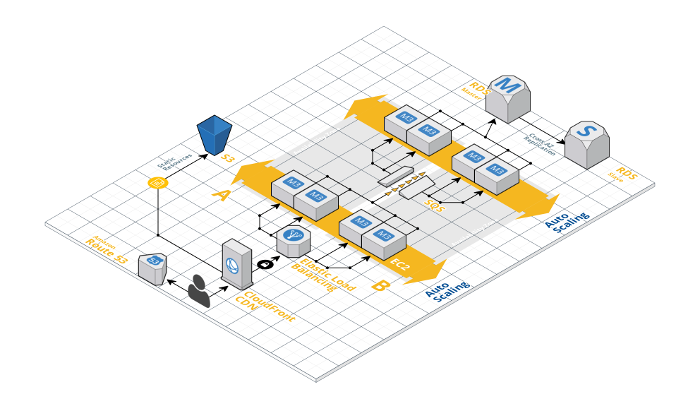
\includegraphics[width=0.8\textwidth]{resources/chapter-2-infrastructure-diagram.png}
        \caption{Contoh gambar}
        \label{fig:1}
    \end{figure}

    \subsubsection{Subsubbab}

    \blindtext
	
	\begin{table}[h!]
		\centering
		\caption{Contoh tabel}
		\begin{tabular}{|c|c|c|c|} 
			\hline
			Col1 & Col2 & Col2 & Col3 \\
			\hline
			1 & 6 & 87837 & 787 \\ 
			\hline
			2 & 7 & 78 & 5415 \\
			\hline
			3 & 545 & 778 & 7507 \\
			\hline
			4 & 545 & 18744 & 7560 \\
			\hline
			5 & 88 & 788 & 6344 \\
			\hline
		\end{tabular}
		\label{table:1}
	\end{table}
	
\section{Studi Terkait}
\blindtext

    \newpage
\chapter{Analisis dan Perancangan} \label{Bab III}

\section{Alur Penelitian} \label{III.Alur}
Digambarkan terkait bagaimana proses yang dilakukan dalam penelitian, dari awal sampai dengan akhir. Gambarkan dalam bentuk diagram alir (\textit{flowchart}). \par

\section{Penjabaran Langkah Penelitian} \label{III.Jabar Alur}
Penjelasan detail dari langkah-langkah alur penelitian, yang sudah tergambar dalam flowchart di subbab \ref{III.Alur}. Subsubbab berikut harus sesuai dengan jumlah alur penelitian. \par

\subsection{Langkah 1} \label{III.Langkah 1}
Penjelasan Langkah 1. \par

\subsection{Langkah 2} \label{III.Langkah 2}
Penjelasan Langkah 2. \par

\section{Alat dan Bahan Tugas Akhir} \label{III.Alat dan Bahan}
Berisi alat-alat dan bahan-bahan yang digunakan dalam penelitian. \par

\subsection{Alat} \label{III.Alat}
Alat yang digunakan untuk melakukan penelitian, dapat berupa computer, PC, Arduino, raspberry, etc. Contoh: \par
\begin{enumerate}[noitemsep]
	\item \textit{Notebook} dengan spesifikasi minumum sistem operasi Windows 11, processor AMD Ryzen 5 7430 CPU @ 6 core/2,3 GHz, RAM 16GB DDR4, grafis AMD Radeon RX Vega 7 2GB, SSD 512 GB.
	\item \textit{Smartphone} dengan spesifikasi OS Android OS 12, CPU Snapdragon 778G Octa-core, GPU Adreno 642L, memori 128 GB, RAM 6 GB.
	\item Platform game engine Godot v4.3
	\item Code editor Microsoft Visual Studio Code
	\item Github
\end{enumerate}

\subsection{Bahan} \label{III.Bahan}
Bahan yang digunakan/diperlukan untuk melakukan penelitian, dapat berupa: \par
\begin{enumerate}[noitemsep]
	\item Dataset pihak lain yang diperoleh dengan izin atau dalam lisensi yang diizinkan untuk digunakan secara langsung,
	\item Dataset pihak pertama yang disusun sendiri melalui quisioner, observasi, atau interview,
	\item Dokumen panduan yang mengacu pada standar, hasil tugas akhir, atau artikel yang disitasi dan digunakan. 
\end{enumerate}

\section{Metode Pengembangan/Pengukuran} \label{III.Metode}
Membahas mengenai metode yang digunakan dalam penelitian, berdasarkan dasar teori yang sebelumnya sudah dijelaskan pada subbab \ref{II.Teori}. Setiap Tugas Akhir wajib memiliki metode dalam pelaksanaannya yang sesuai dengan penelitian yang dikerjakan: \par
\begin{enumerate}[noitemsep]
	\item Alur pengembangan tugas akhir, menggunakan flowchart
	\item Cara pengumpulan data yang digunakan ()Kuesioner, Wawancara, pengujian, dan lainnya)
	\item Metode pengembangan tugas akhir (Metode Waterfall, Agile, RAD, dan lainnya).
\end{enumerate}

\section{Ilustrasi Metode Pengembangan/Pengukuran} \label{III.Ilustrasi}
Jelaskan contoh perhitungan dari metode pengemubangan bagi penelitian Tugas Akhir yang menggunakan algoritma perhitungan tertentu. Tidak perlu harus menggunakan seluruh dataset, cukup menggunakan sampel data. Tujuannya untuk menggambarkan alur perhitungan metode dari data awal sampai luaran yang ditargetkan. \par

\section{Rancangan Pengujian} \label{III.Rancang Uji}
Penjabaran terkait rancangan \& skenario pengujian pada penelitian. Dapat berupa pengujian perangkat keras, lunak, fungsional, dan non-fungsional.
    \newpage
\chapter{Hasil dan Pembahasan} \label{Bab IV}

\section{Hasil Penelitian} \label{IV.Hasil}
Berisi hasil penelitian berdasarkan rancangan yang sudah dijelaskan pada Bab \ref{Bab III}, terutama dari Subbab \ref{III.Metode}. Bagi yang membuat alat, jelaskan alat yang jadi dalam bentuk apa. Bagi yang membuat aplikasi, jelaskan aplikasi yang jadi dalam bentuk seperti apa. Jabarkan dalam bentuk pseudocode dan dijelaskan per bagian kodenya. Gunakan gambar dan tabel sebagai alat bantu menjelaskan hasil. \par

\section{Hasil Pengujian} \label{IV.Uji}
Berikan hasil pengujian berdasarkan rancangan \& skenario yang sudah direncanakan sebelumnya pada Subbab \ref{III.Rancang Uji}. \par

\begin{longtable}{|c|c|c|}
	\caption{Contoh Hasil Pengujian}
	\label{table:4.uji}\\
	\hline
	\textbf{Pengujian} & \textbf{Metode A} & \textbf{Metode B} \\
	\hline
	\endhead
	Kecepatan & 10 ms & 12 ms \\ 
	\hline
	Memori & 10 MB & 7 MB \\
	\hline
\end{longtable}

\begin{figure}[H]
	\centering
	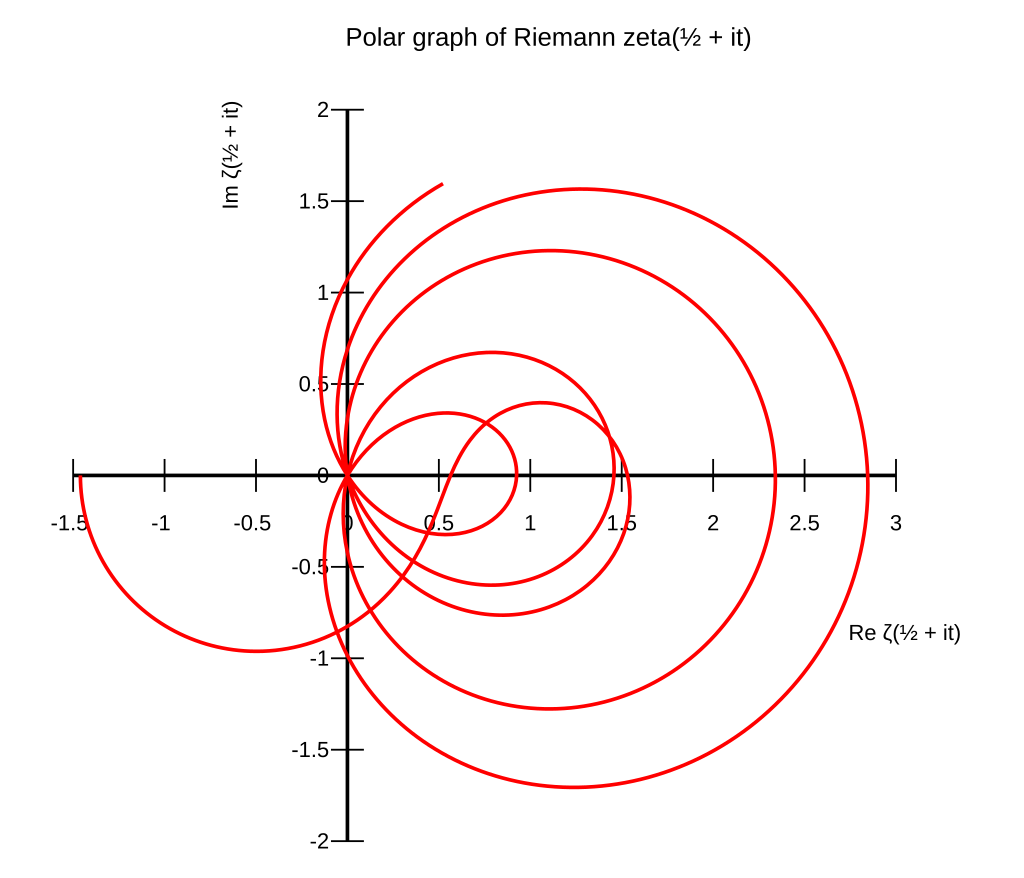
\includegraphics[width=0.5\textwidth]{figure/zeta.png}
	\caption{Contoh Graf Pengujian}
	\label{fig:4.graf}
\end{figure}

\section{Analisis Hasil Penelitian} \label{IV.Analisis}
Berikan analisis hasil penelitian \& pengujian, berupa data yang didapatkan dari penelitian \& pengujian Tugas Akhir yang sudah anda kerjakan. Gunakan gambar dan tabel sebagai alat bantu menjelaskan analisis hasil. Data luaran penelitian yang dapat dianalisis berupa: \par
\begin{enumerate}[noitemsep]
	\item Hasil pengujian
	\item Hasil kuesioner
	\item Aplikasi yang dikembangkan
\end{enumerate}
Analisis dapat membandingkan dengan hasil penelitian sebelumnya yang memiliki kemiripan topik. \par

\section{Pembahasan} \label{IV.Bahas}
Berisi pembahasan terkait hasil yang sudah didapatkan/dipaparkan sebelumnya, berupa penutup yang dapat menjelaskan mengenai kelebihan hasil tugas akhir dan kekurangannya dibandingkan dengan penelitian atau produk lain yang serupa atau mirip. \par
    \newpage
\chapter{Kesimpulan dan Saran} \label{Bab V}

\section{Kesimpulan} \label{V.Kesimpulan}
Berisi kesimpulan dari hasil dan pembahasan terkait penelitian yang dilakukan, dapat juga berupa temuan yang Anda dapatkan setelah melakukan penelitian atau analisis terhadap tugas akhir Anda. Berhubungan dengan poin pada subbab \ref{I.Rumusan Masalah} Rumusan Masalah dan \ref{I.Tujuan} Tujuan. 

\section{Saran} \label{V.Saran}
Berisi saran mengenai aspek Tugas Akhir atau temuan dalam penelitian. Diutamakan saran berdasarkan hasil analisis dari subbab \ref{IV.Analisis}. Saran dapat dikembangkan dan diperkaya untuk Tugas Akhir selanjutnya. 
    %----------------------------------------------------------------%

    % Daftar pustaka
    \renewcommand{\bibname}{Daftar Pustaka}
    \phantomsection% 
    \addcontentsline{toc}{chapter}{Daftar Pustaka}
    \printbibliography

    % Index
    \appendix

    \addcontentsline{toc}{part}{Lampiran}
    \part*{Lampiran}

    \chapter{Instrumen Pengujian}
    \chapter{Rincian Kasus Uji}

\end{document}
